Testy tej części aplikacji składały się~z~weryfikacji czy zaimplementowane~w~aplikacji wzory dla
sensorów pomiarowych zwracają poprawne wartości. Wykonane zostały obliczenia na podstawie teorii,
których wyniki zostały porównane~z~tymi pojawiającymi się~w~aplikacji.~W~tym celu do kodu źródłowego
dodana została specjalna funkcja, która wyświetla wielkości wykorzystywane przez aplikację do
weryfikacji odpowiedzi użytkownika. Wartość ta wyświetla się tylko~w~konsoli przeglądarki, gdy
aplikacja uruchomiona jest na serwerze deweloperskim -- nie ma do niej dostępu~w~wersji produkcyjnej
aplikacji. Dodatkowo przeprowadzone zostały testy czy generowane przez aplikacje produkują
prawidłowe wartości do generowania wykresów oraz czy wykresy te są wykreślone prawidłowo.

Na przykładzie przetwornika LVDT (przedstawionego~w~rozdziale
\ref{sect:theory-lvdt}) wykonane zostały obliczenia dla takiej samej konfiguracji jak wybrana
została~w~aplikacji:
\begin{itemize}
  \item [--]  liczba zwojów~w~uzwojeniu pierwotnym $N_p$ = 1000,
  \item [--]  napięcie wejściowe $U_{wej}$ = 5V,
  \item [--]  częstoliwość napięcia zasilania układu przetwornika $f$ = 1000Hz.
\end{itemize}
Pozostałe wartości zaczerpnięte zostały~z~teorii dostępnej~w~aplikacji. Po zapisaniu
konfiguracji~w~aplikacji zestaw otrzymanych danych (wartości przemieszczenia \textit{\textrm{x}})
to: 0, 7, 9, 3, 15mm. Wartości te generowane są losowo~z~określonego zakresu. Mogą być one
tylko~o~wartości dodatniej, mimo faktu, że rdzeń~w~przetworniku LVDT może poruszać się~w~dwie
strony. Ponieważ charakterystyka przetwarzania sensora jest symetryczna względem punktu równowagi
(co przedstawione zostało~w~rozdziale \ref{sect:theory-lvdt}) zastosowane zostało wyliczanie
wartości dla ujemnych \textit{\textrm{x}} przez funkcje aplikacji. Metoda ta pozwala na otrzymanie
prawidłowego wykresu, który będzie zgodny~z~rzeczywistą charakterystyką przetwarzania. Podstawiając
odpowiednie wartości do wzoru otrzymane zostały następujące wyniki:

\begin{equation*}
  U_{wy} =1000\cdot \frac{5}{10\cdot 10^3}\cdot\bigg(16\pi^2\cdot 0.5\cdot 1000^2\cdot
  10^{-7}\cdot 20\cdot 10^{-3}\cdot\frac{0}{3\cdot 10\cdot 10^{-3}}\cdot\log{(2)}\bigg)
  \bigg(1-\frac{0^2}{2\cdot (20\cdot 10^{-3})^2}\bigg)
\end{equation*}
\begin{equation*}
  \therefore\quad U_{wy} = 0
\end{equation*}

Dla pozostałych wartości przemieszczenia rdzenia:
\begin{align*}
  U_{wy} & =5.2063\approxeq 5.21\quad\text{dla}\quad x=7  \\
  U_{wy} & =6.4085\approxeq 6.41\quad\text{dla}\quad x=9  \\
  U_{wy} & =2.3501\approxeq 2.35\quad\text{dla}\quad x=3  \\
  U_{wy} & =8.5418\approxeq 8.54\quad\text{dla}\quad x=15
\end{align*}

Porównując otrzymane wielkości~z~wynikami, które funkcja drukuje~w~konsoli deweloperskiej, co
przedstawione zostało na rysunku \ref{img:tests-lvdt}, można stwierdzić, że implementacja
wzorów~w~aplikacji jest prawidłowa. Natomiast jeżeli porówna się wygenerowany przez aplikację wykres
dla sensora LVDT, który przedstawiony jest na rysunku \ref{img:graph-lvdt}~z~wykresem teoretycznym,
przedstawionym na rysunku \ref{img:transfer-lvdt}, możliwe jest stwierdzenie, że wykres jest
prawidłowy.

\addimage{0.45}{code/tests-lvdt}{\label{img:tests-lvdt}Wydruk~z~konsoli pokazujący generowane przez
  aplikację wartości}

\addimage{0.7}{app-ui/graph-lvdt}{\label{img:graph-lvdt}Wygenerowany przez aplikację wykres
  zależności dla sensora LVDT}

Wykonane zostały także testy pozostałych ćwiczeń laboratoryjnych. Na podstawie wzorów
przedstwionych~w~rozdziałach \ref{sect:theory-temperature} oraz \ref{sect:theory-strain} obliczono
jakie wartości dla poprawnych odpowiedzi powinny pojawić się~w~konsoli deweloperskiej.

\paragraph{Sensory temperatury:}~W~przypadku termorezystorów metalowych aplikacja wygenerowała
następujące wartości tempertury: 0, 180, 245, 140, 500. Korzystając ze wzoru
\ref{eqn:resistance-rtd} wyznaczone zostały wartości: 100, 167.122, 191.3605, 152.206, 286.45;

Natomiast dla termogniw wylosowane zostały temperatury: 0, 205, 105, 340, 500.
Korzystając~z~równania \ref{eqn:voltage-thermocouple} wyliczono wartości: 0, 10.455, 5.355, 17.34,
25.5;

Porównując otrzymane wyniki~z~wartościami wyznaczonymi przez aplikację, przedstawionymi na
rysunkach~\ref{img:tests-rtd} oraz \ref{img:tests-thermocouple} można stwierdzić, że
generowane przez kod wielkości do weryfikacji odpowiedzi są prawidłowe.

\begin{figure}[!htbp]
  \hfill
  \subfloat[][Wyniki dla ćwiczenia z
    termorezystorami]{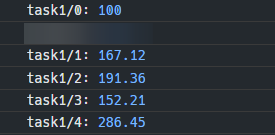
\includegraphics[width=0.45\textwidth]{code/tests-rtd}\label{img:tests-rtd}}
  \hfill
  \subfloat[][Wyniki dla ćwiczenia z
    termoogniwami]{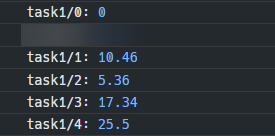
\includegraphics[width=0.45\textwidth]{code/tests-thermocouple}\label{img:tests-thermocouple}}
  \hfill
  \caption{\label{img:calc-console-temperature}Wydruk~z~konsoli pokazujący generowane przez
    aplikację wartości}
\end{figure}

Na przykładzie termorezystorów zweryfikowane zostało generowanie charakterystyk dynamicznych dla
sensorów temperatury. Na rysunku \ref{img:graph-temperature-dynamic} przedstawiony został wykres,
który stworzyła aplikacja. Porównując go do przykładowego wykresu odpowiedzi skokowej
(przedstawionego na rysunku \ref{img:dynamic-characteristic}) widać, że jest to wykres
zgodny~z~teorią.

\addimage{0.6}{app-ui/graph-temperature-dynamic}{\label{img:graph-temperature-dynamic}Wygenerowany
  przez aplikację wykres charakterystyki dynamicznej dla termorezystora metalowego}

\paragraph{Tensometry:} Aby zweryfikować poprawność wyników generowanych przez aplikację należało
wyznaczyć wartości napięcia na wyjściu mostka. Sprawdzony został przypadek gdy nie bierze się pod
uwagę wpłwu temperatury na pracę układu. Do obliczeń wykorzystano równanie \ref{eqn:quater-bridge}
przy czym nie brana była pod uwagę składowa~z~temperaturą. Dla zadania generowane są wartości
odkształcenia jakim poddawne są tensometry, aplikacja wylosowała następujące wartości: 3, 2.2,
1.6, 2.5, 1.9; Wykonując obliczenia otrzymano następujące wartości: 9.75, 7.15, 5.2, 8.125, 6.175;

Porównując otrzymane wyniki~z~wartościami wyznaczonymi przez aplikację, przedstawionymi na
rysunku~\ref{img:tests-strain-no-temp} można stwierdzić, że generowane odpowiedzi są prawidłowe.
Na rysunku \ref{img:graph-strain} widać, że generowany przez aplikację wykres odzwierciedla wzrost
napięcia na wyjściu układu wraz~z~rosnącą wartością odkształcenia.

\addimage{0.45}{code/tests-strain-no-temp}{\label{img:tests-strain-no-temp}Wydruk~z~konsoli
  pokazujący generowane przez aplikację wartości}

\addimage{0.7}{app-ui/graph-strain}{\label{img:graph-strain}Wykres przedstawiający zależność
  napięcia wyjściowego od wartości odkształcenia}